\documentclass[11pt,oneside,a4paper]{article}
\usepackage{graphicx}
\usepackage{hyperref}

\title{Hello}


\title{Integrating Knowledge Graphs into the Debian Ecosystem}
\author{Alexander Belikov \\ \href{mailto:alexander@growgraph.dev}{alexander@growgraph.dev}}
\date{June 2025}

\begin{document}

    \maketitle

    \begin{abstract}
        In an era where software systems are increasingly complex and interconnected, understanding and managing the relationships between packages, maintainers, dependencies, and vulnerabilities is paramount.
        We propose the innovative integration of knowledge graphs into the Debian ecosystem, offering a structured and semantic approach to package management and analysis.
        We examine how knowledge graphs can unify heterogeneous data sources — including package metadata, security advisories, and reproducibility reports — into a coherent model that enhances visibility, enables multi-hop reasoning, and supports optimization suggestions beyond the capabilities of traditional relational or document‑oriented systems.

    \end{abstract}


    \section{Introduction}
    Knowledge graphs (KGs), with roots in the semantic web, have achieved widespread adoption — from powering search engines and question‑answer systems to enabling analytics in domains such as healthcare, finance, and smart cities~\cite{Iliadis2023-cm}.
    Their potential in software ecosystems is gaining momentum, where they facilitate the integration of package metadata, security vulnerabilities, license data, and build information into a unified semantic framework.

    The Debian distribution, comprising over 50,000 packages and a global community of contributors, exemplifies a richly interconnected software ecosystem.
    Packages depend upon one another, maintainers contribute expertise in particular subsystems, security updates propagate through dependency chains, and reproducible builds underpin software trust.
    However, traditional tabular or textual representations struggle to surface complex, multi‑hop relations — such as tracing vulnerability exposure through nested dependencies or uncovering maintainer centrality within specialized domains.

    A knowledge graph approach offers several compelling advantages.
    First, it enables rapid identification of downstream packages affected by a specific vulnerability — critical for timely patch deployment.
    Second, it supports auditing of license compatibility by traversing transitive dependencies to detect potential conflicts between GPL, LGPL, or proprietary licenses.
    Third, KG‑based analysis can surface maintainership expertise networks, revealing specialists in areas like networking or GUI toolkits and informing mentorship and delegation strategies.
    Fourth, by integrating reproducibility results — such as build metadata from reproducible builds infrastructure — the graph can highlight clusters of packages lacking reproducibility, enabling targeted community intervention.
    Finally, linking external signals (e.g.\ feature‑request platforms or “grow your ideas” proposals) to Debian packages and maintainers provides data‑driven insight into unmet feature needs and community engagement opportunities.

    In this paper, we present \emph{Deb‑KG}, a knowledge graph for the Debian ecosystem.
    Constructed using the GraphCast ingestion framework~\cite{graphcast}, Deb‑KG integrates package metadata, security advisories, reproducibility reports, and external community signals into a property‑graph model.
    We describe its schema, ingestion pipeline, and demonstrate use cases including vulnerability tracing, license compliance auditing, maintainer profiling, reproducibility monitoring, and community‑informed prioritization.

    At the same time it is a complex ecosystem, interconnected at many levels.

    It is critical to optimize debian workflow not only from the point of view of saving time, but also direct towards updates in most critical areas, reduce uncertainty about future updates, enhance robustness.
    Connect external data sources to learn (some bugs are not reported) which way to direct it.


    Importance of implicit interactions between code and people (often unique expertise).


    \section{Related Work}


    \section{Schema}

    \begin{figure}[h]
        \centering
        \begin{tabular}{cc}
            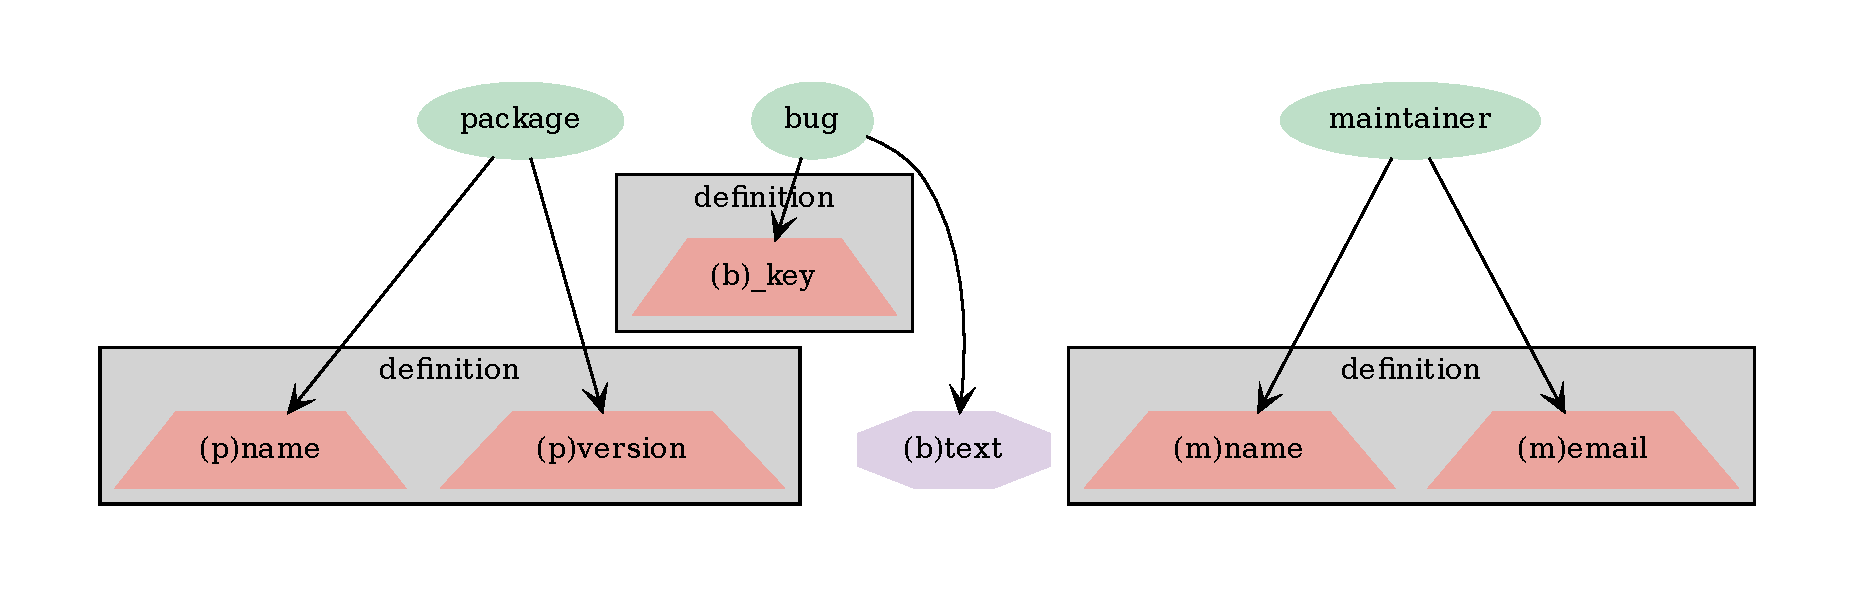
\includegraphics[width=0.8\textwidth]{../figs/debian-eco-vc2fields} &
            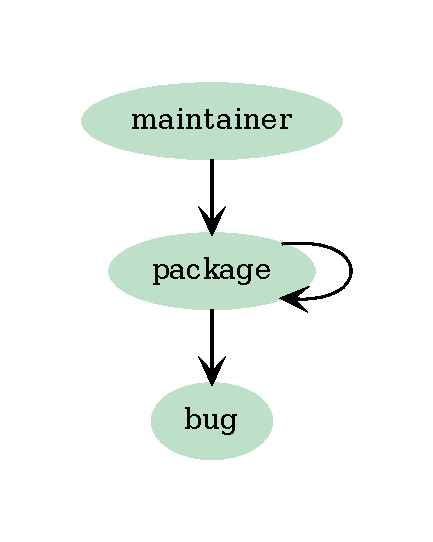
\includegraphics[width=0.2\textwidth]{../figs/debian-eco-vc2vc} \\
        \end{tabular}
        \caption{\textbf{Left}: \textbf{Right}:.}\label{fig:schema}
    \end{figure}


    Represent as a property graph.

    Use GraphCast for processing: <https://growgraph.github.io/graphcast/>.

    A framework for transforming tabular (CSV, SQL) and hierarchical data (JSON, XML) into property graphs and ingesting them into graph databases (ArangoDB, Neo4j).

    Describe relations: package, maintainer, dependencies, bugs.


    \section{Use Cases}

    Enhanced Use Cases:

    - Tracking and validating package dependencies.
    - Identifying and analyzing vulnerability propagation.
    - Assessing license compatibility and compliance.
    - Auditing build reproducibility across packages.
    - Highlighting Areas Lacking Reproducible Builds.
    - Mapping Community Needs: Linking data from platforms like "grow-your-ideas" with package metadata to identify areas lacking attention
    - Informing Funding Decisions: Providing data-driven insights to allocate resources effectively, ensuring that critical community needs are addressed.

    Community Collaboration: Understand how this approach can foster collaboration within the Debian community, providing tools for maintainers, developers, and researchers to contribute and benefit from shared insights.


    \section{Conslusion}


    Present in this repository:
    https://github.com/alexander-belikov/deb-kg

    \bibliographystyle{plain}
    \bibliography{refs}

\end{document}
